
%% No past tense or passive writing
\chapter{ConFrm}
We build ConFrm to address the challenges that ...


\section{Specification: Relatively Deterministic Noninterference}
ConFrm modifies data noninterference to address the non-uniform outcome probabilities challenge. In the following part we will progressively build our specification that addresses this challenge. 

\subsection{Basic Definition}
One way to solve the problem is ensuring that a program has the same return value if  same nondeterministic events happen during executions from related states. Since each execution corresponds to a specific set of nondeterministic events, aforementioned requirement prevents choosing the same execution multiple times to satisfy noninterference. Therefore such requirement ensures the existence of a 1-to-1 pairing between executions from equivalent states. Existence of a 1-to-1 pairing for executions implies that the distribution of the observed return values is preserved between equivalent states. This requirement is indeed sufficient to address our problem. Figure \ref{fig:RDNI_Matching_Paths} visualizes how the example \ref{fig:Frequency_Leaking_Program} does not satisfy the new requirement, although it satisfies the conventional definition. There is no corresponding execution from the related state if the first generated random bit is 1.

\begin{figure}[h]
    \centering
    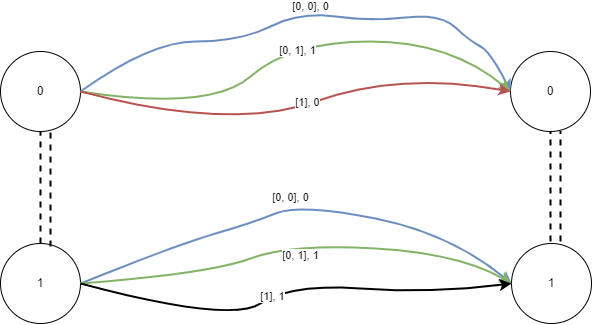
\includegraphics[scale=0.5]{templates/figures/matching-paths-rdni.png}
    \caption{There is no corresponding execution for the red and black executions.}
    \label{fig:RDNI_Matching_Paths}
\end{figure}

We formalized the notion described above to a new definition called relatively deterministic noninterference (RDNI). First modification we made was to the execution relation. ConFrm provides an execution relation that takes a source of nondeterminism, which we call an oracle, and refers to it whenever it needs to make a nondeterministic choice, e.g. crashing or successfully executing. One important requirement is that oracle has to capture all the nondeterminism in the system. In other words, if we fix an oracle, execution should be deterministic. Since all possible nondeterminism in the system is captured by the oracle, it is possible to reason about specific series of nondeterministic events by reasoning about the oracle itself. Figure \ref{fig:RDNI_no_recovery} shows the formalization of this approach.

%Footnote between relations and equivalences
\begin{figure}[ht]
    \centering
    \begin{verbatim}
    Definition simple_RDNI
        {T} (u: user) (p: prog T)
       (R: state -> state -> Prop) :=
      forall (o: oracle) (s1 s2: state) (res1: Result T),
        exec u o s1 p res1 ->
        R s1 s2 ->
        exists res2, 
            exec u o s2 p res2 /\
            R (extract_state res1) (extract_state res2) /\
            extract_ret res1 = extract_ret res2.
    \end{verbatim}
    \caption{Simple relatively deterministic noninterference.}
    \label{fig:RDNI_no_recovery}
\end{figure}

\subsection{Crash, Reboot, and Recovery}
\paragraph{Crashes.}
Since we will be reasoning with crash-safe systems, ConFrm provides support for crashes, reboots and a recovery. 
We defined two different execution results in ConFrm to support crash semantics of a system: \texttt{Finished}, and \texttt{Crashed}. A \texttt{Finished} result means that program is successfully completed and contains a state and a return value. A \texttt{Crashed} result means that the system crashed in the middle of the execution and contains only a state, which represents the state of the system after the crash happened but before rebooting.

Crash semantics of the system are defined by the developer as they are defining their system model. It is developer's responsibility to ensure that defined execution semantics are correctly capturing the system behavior.

\paragraph{Reboots.}
Reboot process can also be a source of nondeterminism in the system. One example of this is an asynchronous disk. When a system crashes and reboots, the disk can be in one of the multiple possible states due to buffered and reordered writes. To capture and quantify this source of nondeterminism, we introduced reboot state functions - or reboot functions for short. A reboot function takes a state after a crash and returns the state that the system will be after a reboot. Just like the crash semantics, it is the developer's responsibility to ensure that their reboot function accurately models the behavior of their system.

We chose to separate the definition of the reboot functions from the definition of the system. Reason for our choice was to not constrain the developer to a single function definition. Ability to reason about different reboot functions was essential to capture reboot behavior of an asynchronous disk.

\paragraph{Recovery.}
Recovery semantics for systems are provided by ConFrm and added automatically when a language is generated from a core. To distinguish these semantics from the semantics of the execution of a single program, we will refer to recovery semantics as executing-with-recovery. In ConFrm's recovery model, only two outcomes are possible when executing-with-recovery: (1) execution can finish without any crashes, or (2) execution crashes then recovers after certain number of attempts. To represent these two outcomes, ConFrm uses two types of recovery result: \texttt{RFinished} and \texttt{Recovered}. \texttt{RFinished} corresponds to the case (1) and \texttt{Recovered} corresponds to the case (2).
Since there is no rule for crashing infinitely many times, provided semantics implicitly assume that recovery eventually will succeed. 

Semantics for (1) is straightforward. If the program successfully executes, then it successfully executes-with-recovery.
Semantics for (2) is more involved. They are inductively defined to capture repeated attempts of recovery until it succeeds. It states that if the original program crashes, and recovery program executes-with-recovery to some result, then original program executes-with-recovery to the state of that result. Since semantics require running many programs with multiple crashes, execution relation takes a list of oracles and a list of reboot functions. An oracle and a reboot function is used every time a crash happens. Therefore, length of those lists implicitly determines how many times the recovery will crash until it succeeds. Formalized semantics can be seen in figure \ref{fig:Recovery_Semantics}


\begin{figure}[ht]
    \centering
    \begin{verbatim}
Inductive exec_with_recovery :
forall T, user -> list oracle -> state -> 
list (state -> state) -> prog T -> prog unit -> 
@Recovery_Result state T -> Prop :=
    | ExecFinished :
      forall T (p: prog' T) p_rec
        u o d d' t,
        exec u o d p (Finished d' t) ->
        exec_with_recovery u [o] d [] p p_rec (RFinished d' t)
    | ExecRecovered :
      forall T (p: prog' T) p_rec
        u o lo d d' get_reboot_state l_grs ret,
        exec u o d p (Crashed d') ->
        exec_with_recovery u lo (get_reboot_state d') 
            l_grs p_rec p_rec ret ->
        exec_with_recovery u (o::lo) d (get_reboot_state::l_grs) 
            p p_rec (Recovered (extract_state ret)).
    \end{verbatim}
    \caption{Recovery semantics in ConFrm}
    \label{fig:Recovery_Semantics}
\end{figure}

We incorporated executions with recovery into RDNI definition to create a noninterference statement that encompasses the entire crash-reboot-recover cycle. We also changed \texttt{extract\_ret} to return an option type to distinguish between \texttt{RFinished} and \texttt{Recovered} results. This change ensured that both results will have the same result type. Figure \ref{fig:RDNI_recovery} shows the formalization with recovery executions.

\begin{figure}[ht]
    \centering
    \begin{verbatim}
Definition RDNI_with_recovery
    {T} (u: user) (p: prog T) 
    (rec: prog unit)
    (R: state -> state -> Prop) :=
  forall (l_o: list oracle) 
  (l_rf: list (state -> state))
  (s1 s2: state) (res1: Result T),
    exec_with_recovery u l_o s1 l_rf p rec res1 ->
    R s1 s2 ->
    exists res2,
        exec_with_recovery u l_o s2 l_rf p rec res2 /\
        R (extract_state res1) (extract_state res2) /\
        extract_ret res1 = extract_ret res2.
    \end{verbatim}
    \caption{RDNI with recovery executions.}
    \label{fig:RDNI_recovery}
\end{figure}

We made two more addition to RDNI to unify \texttt{state\_noninterference} and \texttt{ret\_noninterference} into a single definition. First, we made return value equality conditioned on a predicate for the user being true. This way, we can require return value equivalence to hold only for the users that the states are equivalent for. Second, we made it so it is defined over two programs. This change was needed because ConFrm programs contain their input arguments and we needed to be able to reason about a function executing with different input arguments. With these changes, we reach our final definition for RDNI, which is shown in Figure \ref{fig:RDNI_final}.

\begin{figure}[ht]
    \centering
    \begin{verbatim}
    Definition RDNI_with_recovery
        {T} (u: user) (p1 p2: prog T) 
        (rec: prog unit)
       (R: state -> state -> Prop) 
       (cond: user -> Prop):=
      forall (l_o: list oracle) (l_rf: list (state -> state))
      (s1 s2: state) (res1: Result T),
        recovery_exec u l_o s1 l_rf p1 rec res1 ->
        R s1 s2 ->
        exists res2,
            recovery_exec u l_o s2 l_rf p2 rec res2 /\
            R (extract_state res1) (extract_state res2) /\
            (cond u -> extract_ret res1 = extract_ret res2).
    \end{verbatim}
    \caption{Final definition of RDNI}
    \label{fig:RDNI_final}
\end{figure}

{\color{red}
\subsection{Termination Sensitivity}}

% This is ConFrm so rename it
\section{Proof Approach}
Our proof approach consists of two parts. First part is the support for abstraction. Second part is the meta-theory that provides relevant theorems to prove confidentiality of implementation from the confidentiality of abstraction. We will first present the infrastructure for defining abstractions then explain the meta-theory.

\subsection{Cores, Languages, and Refinements}
\paragraph{Cores.}
ConFrm introduces cores as the main way to model the system and the languages. A core has four components. First one is the state that will be used in operational semantics. Second one is list of possible operations (opcodes). Third one is list of possible nondeterminism tokens. Nondeterminism tokens are how we implement the concept of oracles from RDNI. Fourth one is the execution semantics of each operation.

Also, to ensure that tokens capture all the nondeterminism in the semantics, a proof that shows, given a token, execution semantics are deterministic is required.

\begin{figure}[ht]
    \centering
    \begin{verbatim}
Record Core :=
  {
    token : Type;
    state : Type;
    operation : Type -> Type;
    exec: forall T, user -> token -> state ->
        operation T -> @Result state T -> Prop;
    
    exec_deterministic_wrt_token :
      forall u o s T (p: operation T) ret1 ret2,
        exec u o s p ret1 ->
        exec u o s p ret2 ->
        ret1 = ret2;
  }.
    \end{verbatim}
    \caption{Definition of a core}
    \label{fig:Core_Definition}
\end{figure}

\paragraph{Languages.}
ConFrm also includes the machinery that turns a core to a full language by equipping it with a computation monad. This prevents the repetitive work that needs to be done to define languages. It also allows framework to provide core-agnostic theorems and tactics to be used in proofs.

Semantics of the language are derived from the semantics of its core. New  semantics takes a list of tokens (i.e. an oracle) and consumes exactly one at each step. Turning a core into a language also gives it its recovery semantics.

ConFrm also provides some theorems regarding determinism of an execution as well as relationship between oracles and executions like how two executions relate to each other if one's oracle is a prefix of the other's.

\paragraph{Refinements.}
ConFrm's main mechanism for relating abstractions and implementations is refinements. 
ConFrm defines a refinement as an object between an implementation language and a core abstracting it. We had to extend the standard refinement definition to accommodate both crashes and oracles.

A refinement has four components that corresponds the four components of a core, and a theorem states that a successful execution preserves the state refinement relation. These components are
\begin{itemize}
    \item a \texttt{compile} function, that turns an  abstract operation to its implementation program,
    \item a \texttt{refines} relation that relates an abstract state to an implementation state,
    \item a \texttt{refines\_reboot} relation that relates an abstract reboot state to an implementation reboot state,
    \item and  \texttt{token\_refines} relation that relates an abstract token to an implementation oracle.
\end{itemize}

\begin{figure}[ht]
    \centering
    \begin{verbatim}
Record CoreRefinement {O_imp} (L_imp: Language O_imp) (O_abs: Core) :=
  {
    compile_core : forall T, O_abs.(Core.operation) T -> L_imp.(prog) T;
    
    refines_core: L_imp.(state) -> O_abs.(Core.state) -> Prop;
    
    refines_reboot_core: L_imp.(state) -> O_abs.(Core.state) -> Prop;
    
    token_refines: forall T, user -> L_imp.(state) -> 
        O_abs.(Core.operation) T -> (L_imp.(state) -> 
        L_imp.(state)) -> L_imp.(oracle) -> 
        O_abs.(Core.token) -> Prop;
    
    exec_compiled_preserves_refinement_finished_core :
      forall T (p2: O_abs.(Core.operation) T) o1 s1 s1' r u,
        (exists s2, refines_core s1 s2) ->
        L_imp.(exec) u o1 s1 (compile_core T p2) (Finished s1' r) ->
        (exists s2', refines_core s1' s2');
  }.
    \end{verbatim}
    \caption{Definition of a core refinement}
    \label{fig:Core_Refinement_Definition}
\end{figure}

Both \texttt{compile} and \texttt{refines} are part of the standard definition. However \texttt{refines\_reboot} and \texttt{token\_refines} relations require more explanation.

We had to separate \texttt{refines\_reboot} from \texttt{refines} because, in general, \texttt{refines} relation was too strong to hold for after-reboot states but we also needed a relation between them to ensure that recovery restores the original \texttt{refines} relation.

\texttt{token\_refines} relation is more complicated. On top of the oracle and the token it relates, it takes the following as parameters
\begin{itemize}
    \item a user,
    \item an implementation state,
    \item an abstract operation,
    \item and an implementation reboot function.
\end{itemize}
All these parameters were necessary to capture intricate relationship between abstract tokens and implementations' crash and recovery behavior. We can demonstrate the roles they play by examining the following example.

Assume that we are abstracting an implementation of a checksum-based log on an asynchronous disk with a \texttt{write} function.
A crash during a write to a checksum-based log may leave in such a state that whether the \texttt{write} succeeded or not would depends on which blocks made it to the disk before crash happened (which is determined by the after-reboot state of the implementation). In other words, success of a write after crash depends on (1) state of the disk just after the crash, and (2) state of the disk after reboot. To determine (1), we need to know the user, the starting state, and data being written - which is contained in the operation. To determine (2), we need to know the reboot function. Therefore, capturing the behavior of the write in this particular case requires all the parameters listed above. Other operations may require some or all of those parameters as well.

{\color{red} Maybe a figure that demonstrates above paragraph goes here.}

Just like languages, ConFrm can automatically generate a refinement between two languages given a core refinement between an implementation language and an abstraction core. A refinement for a language differs from a refinement in three places. First, \texttt{compile} function transforms programs from the abstraction language to implementation language. Second, \texttt{token\_refines} turns into \texttt{oracle\_refines}, which relates an abstract oracle and an implementation oracle.
Third, a finished execution of any compiled program should preserve the refinement. ConFrm also provides \texttt{recovery\_oracles\_refine} relation, which relates list of implementation oracles to list of abstraction oracles by \texttt{oracle\_refines} inductively.

\paragraph{Horizontal Compositions.}
To enable modular implementations, ConFrm provides automatic derivation of a new, composite core from two given cores via horizontal composition. State of the composite core is a pair that contains the state of each the component cores. This capability allows developers to develop the system in small, self contained parts that can be combined at will when desired without much overhead. A language derived from a composite ConFrm contains support for "lifting" the programs written in a language of the one of the component cores to the language of the composite core. Similarly, it allows automatic derivation of a refinement between the two composite languages if a component of first language is a refinement of a component of the second language.

\subsection{Deriving confidentiality of an implementation}
At the heart of ConFrm lies the theorem which derives the confidentiality of a compiled program from the confidentiality of its abstraction. Theorem reveals the conditions that needs to hold for preserving RDNI through refinement. We identified two such conditions. First condition is about an abstraction capturing all necessary behavior of an implementation. Second one is about independence of abstract nondeterminism from confidential data. More precisely, these two conditions are

\begin{enumerate}
    \item there should be a simulation between implementation and abstraction with respect to refinement relations, and
    \item if a list of implementation oracles refine a list of abstract oracles from a state with the first program, then it should refine the same oracle from any state that is related to the first state with the second program.
\end{enumerate}

First condition ensures that there is no execution of a compiled program that is not captured by an execution of an abstract program. This is necessary for a property of any abstract execution to imply a property of any implementation execution. If there was an implementation execution that does not correspond to an abstract execution, then it would not be possible to reason about such execution through an abstract execution.

Second condition can be interpreted as the necessity that abstraction does not inject dependency to the confidential data into abstract oracles. Abstractions modelling some deterministic behaviors of an implementation as nondeterminism is a common pattern. This property makes sure that developer does not abstract a behavior that depends on the confidential data in such a way. If such action would be permitted, then two implementation executions from related states with the same implementation oracles could correspond to two abstraction executions with different oracles.

In such a case, the noninterference of the abstraction with the same oracles wouldn't be strong enough to establish the same fact in implementation, due to the fact that noninterference of the abstraction does not state anything about executions with different oracles.

\paragraph{Simulations.}
First condition states that a simulation must exist between the abstraction and the implementation. Since we introduced oracles and crash-and-recovery into execution relations, we had to modify the standard simulation definition to accommodate those changes. 

First change is that, our modified simulation definition has three simulation relations, one for the starting states, one for the end states and one for the oracles. We had to separate the relation that relates the starting and end state to be able to reason about recovery where the relation that holds at the beginning and at the end are different. 

In our case, they were \texttt{refines\_reboot} and \texttt{refines} relations, respectively. However we also defined a two relation variant to use in transfer theorem's definition, where start and end relations are both \texttt{refines} relation.

Second change is that it is defined over an entire execution-with-recovery. This allows simulation relation to be broken temporarily after a crash, as long as it is restored by the recovery process. This change was necessary because crashes may expose states that will never appear during normal execution. This way, refinement relation can only consider the states that appear during normal execution. How to represent crash states are entirely left to the developer. Formal definition of a simulation can be found in figure \ref{fig:Simulation_Definition}. In implementation, we separated existence of a list of abstract oracles and existence of an abstract execution separate to shorten the proof scripts for individual theorems.   

\begin{figure}[ht]
    \centering
    \begin{verbatim}
Definition SimulationForProgram
   u T (p_abs: L_abs.(prog) T) (rec_abs : L_abs.(prog) unit)
   l_get_reboot_state_imp
   l_get_reboot_state_abs
   R_begin R_end :=
   
  forall l_o_imp s_imp  s_imp' s_abs,
    R_begin s_imp s_abs ->
   L_imp.(exec_with_recovery) u l_o_imp s_imp
    l_get_reboot_state_imp (R.(compile) p_abs)
    (R.(compile) rec_abs) s_imp' ->
    exists l_o_abs s_abs',
        recovery_oracles_refine u s_imp p_abs rec_abs l_get_reboot_state_imp l_o_imp l_o_abs /\
        L_abs.(exec_with_recovery) u l_o_abs s_abs l_get_reboot_state_abs p_abs rec_abs s_abs' /\
        R_end (extract_state_r s_imp') (extract_state_r s_abs') /\
        extract_ret_r s_imp' = extract_ret_r s_abs').
\end{verbatim}
    \caption{Our simulation relation with oracles and execution-with-recovery}
    \label{fig:Simulation_Definition}
\end{figure}



\iffalse 
\begin{figure}[ht]
    \centering
    \begin{verbatim}
Lemma RDNI_Weak_transfer:
  forall O_imp O_abs (L_imp: Language O_imp) (L_abs: Language O_abs) 
    (R: Refinement L_imp L_abs)
    u T (p1_abs p2_abs: L_abs.(prog) T) rec_abs
    l_get_reboot_state_imp
    l_get_reboot_state_abs
    equivalent_states_abs cond,

    RDNI_Weak
      u p1_abs p2_abs rec_abs
      equivalent_states_abs
      cond l_get_reboot_state_abs ->
    
    SimulationForProgram R 
      u p1_abs rec_abs 
      l_get_reboot_state_imp
      l_get_reboot_state_abs ->

    SimulationForProgram R 
      u p2_abs rec_abs 
      l_get_reboot_state_imp
      l_get_reboot_state_abs ->
    
    oracle_refines_same_from_related R 
      u p1_abs p2_abs rec_abs 
      l_get_reboot_state_imp 
      equivalent_states_abs ->
    
    RDNI_Weak
      u (R.(compile) p1_abs)
      (R.(compile) p2_abs)
      (R.(compile) rec_abs)
      (refines_related R equivalent_states_abs)
      cond l_get_reboot_state_imp.
Proof.
\end{verbatim}
    \caption{RDNI transfer theorem}
    \label{fig:RDNI_Transfer_Definition}
\end{figure}


\section{Property Transfers}

\subsection{RDNI transfer}
- Required properties

-- SimulationForProgram
    
-- abstract oracles exist wrt (AOE)

-- oracle refines same from related (ORS)

-- exec compiled preserves validity (Trivial in our case because all of our top states are valid)

-- Termination Sensitive (TS)

\subsection{ORS}
-- have same structure (program flow equivalence) (HSS)

\begin{minted}{coq}
Lemma token_refines_finished_prefix_eq:
forall ...,

token_refines u s1 op1 grs1 o1 t1 ->
token_refines u s2 op2 grs2 o2 t2 ->

exec u s1 o1 (compile op1) (Finished s1' r1) ->
exec u s2 o2 (compile op2) (Finished s2' r2) ->

have_same_structure op1 op2 -> 

(exists s1a,refines s1 s1a) ->
(exists s2a, refines s2 s2a) ->

one_prefix_of_other o1 o2 ->
o1 = o2 /\ t1 = t2.
\end{minted}

\begin{minted}{coq}
Lemma token_refines_crashed_prefix_eq:
forall ...,

token_refines u s1 op1 grs1 o1 t1 ->
token_refines u s2 op2 grs2 o2 t2 ->

exec u s1 o1 (compile op1) (Crashed s1') ->
exec u s2 o2 (compile op2) (Crashed s2') ->

have_same_structure op1 op2 -> 

(exists s1a,refines s1 s1a) ->
(exists s2a, refines s2 s2a) ->

one_prefix_of_other o1 o2 ->
t1 = t2.
\end{minted}

\begin{minted}{coq}
Lemma oracle_refines_impl_eq:
forall ...,
    oracle_refines u s1 p1 imp_reboot_f o1 oa1 ->
    oracle_refines u s2 p2 imp_reboot_f o2 oa2 ->
    
    refines s1 s1a ->
    refines s2 s2a ->
    
    exec u o1 s1 (compile p1) (Finished s1' r1) ->
    exec u o2 s2 (compile p2) (Finished s2' r2) ->
    
    have_same_structure p1 p2 u s1a s2a ->
    
    token_refines_finished_prefix_eq ->
    
    one_prefix_of_other o1 o2 ->
    not_init p1 ->
    not_init p2 ->
    
    o1 = o2 /\ oa1 = oa2.
\end{minted}

\begin{minted}{coq}
Lemma oracle_refines_independent_from_reboot_function:
forall ...,
    exec u o s (compile p) (Finished s' r) ->
    oracle_refines u s p grs o o_abs ->
    forall grs', 
      oracle_refines u s p grs' o o_abs.
\end{minted}

\begin{minted}{coq}
Lemma oracle_refines_prefix_finished_not_crashed:
forall ...,
    oracle_refines u s1 p1 imp_reboot_f o1 oa1 ->
    oracle_refines u s2 p2 imp_reboot_f o2 oa2 ->
    
    refines s1 s1a ->
    refines s2 s2a ->
    
    exec u o1 s1 (compile p1) (Finished s1' r1) ->
    exec u o2 s2 (compile p2) (Crashed s2') ->
    
    have_same_structure p1 p2 u s1a s2a ->
    
    one_prefix_of_other o1 o2 ->
    not_init p1 ->
    not_init p2 ->
    False.
\end{minted}

These are compositional in the sense that proving corresponding properties for 
each operation implies it is true for all programs created from them. 

\subsection{AOE}
\fi